\chapter{Implementation}
\label{cha:implementation}

After shaping a basic theoretical approach and probably sketching different considerations, it is time to define the needed tools and setting up a project repository. Also, it has to be considered, that the finished project should depend on as little third-party software as possible, but also be as deployable as possible.

At the very beginning, a clear structure has to be adopted, which concurrently serves as navigation guide for later development. Having a folder structure ready at development start, it may seem rigid and even narrow down the developer's freedom in creating his/her part of the application logic during some part of the process, but nevertheless it is definitely an important and easy supporting tool for projects being maintained using an asynchronous collaboration workflow. Furthermore, it may even help in creating tasks focusing on certain parts of the development process.

\section{Foundation}
\label{sec:foundation}

Since Node.js is very suitable for providing an instant development environment on most popular operating systems\footnote{\url{http://nodejs.org/dist/latest/} -- Precompiled versions of the latest Node.js release, for different operating systems.}, as well as quickly leveraging a basic application, which provides immediate feedback to its creator -- without depending on any precompilation steps -- it may be considered as basic framework for any further development.

Together with the achievements of ES6, a clean code foundation marks the base structure for further module introduction into the project. Step by step, a modular web service is going to be raised and formed according to its designed operation mode.

\subsection{Express.js for REST}
\label{sec:foundation-express}
Starting with Express.js, the sample code in chapter \ref{sec:primarythoughts-restapi} on p. \pageref{sec:primarythoughts-restapi} gives a good example on how to easily provide an API endpoint. While the example only returns a string containing ``Hello World!'', a JSON structure may also be used and is probably a better choice for working programmatically on the response data later on.

Furthermore, a good advice would be to use a modular form of route definitions, since the main source file will soon get too bloated and may grow a lot of spaghetti-code in it. This may be achieved in outsourcing the routes in specific files and/or folders and importing them via a \emph{require}-statement. As a bonus, an external source file containing route definitions also allows for custom logic and middlewares, which may be hidden to the rest of the application by default \cite[p. 220f]{cantelon2017node}.

\subsubsection{Middleware}
Especially when depending on advanced application logic (e.g. user authentication, database management, etc\ldots), further tasks containing validation checks or user definitions may get necessary. If these tasks are required by more than one route, it makes sense to abstract their logic into reusable components for use as middleware in these specific routes \cite[223]{cantelon2017node}. Optionally, more than one middleware may be used on a single route, where their placement stands for their execution order -- from first to last.

\lstinputlisting[label={list:express-middleware}, language=JavaScript, caption={An example for middleware ordering, where \emph{firstMiddleware} gets called right before \emph{secondMiddleware}. Both middlewares have to succeed (e.g. return \emph{done}-callback function) in order to grant access to the ``/secret'' route.}]{chapters/05-implementation/_support/middleware.js}

\subsubsection{OAuth 2.0}
\emph{OAuth 2.0} stands for an open authorization framework, which grants limited access to a certain HTTP service, either on behalf of a resource owner (e.g. allow access to user data of a social network account), or by allowing a third-party application to obtain access on its own behalf \cite[1]{hardt2012oauth}. In this case, the latter is more interesting, as a programmatical access may be achieved by issuing an access token via a ``client credentials'' grant type. Therefore, an application-only access is possible without depending on any user interaction.

The whole authentication process is necessary, as the final web application will hold different user accounts, as well as their registered projects. Thus, every client (human or non-human) may interact with the application's API only via certain issued tokens, which ideally are only valid for a specific amount of time before they expire \cite[43]{hardt2012oauth}.

\subsubsection{MongoDB}
Every account or project data has to be stored on a non-volatile type of memory to faithfully provide any requested information at any desired point in time. Moreover, these data requests may not interfere with each other, nor cause inconsistencies or conflicts within the storage, even if accessed at the same time. As a consequence, a memory solution depending on files will not likely fulfill every crucial requirement, especially when a service is constantly and fast growing.

A good choice may therefore be to use \emph{MongoDB}, since it stores the entries already as formatted JSON and is not dependent on a fixed table schema beforehand. As a result, the structure most likely does not have to be excessively administered during development and stays as adaptive as possible until a final schema has evolved.

\section{Structure}
\label{sec:structure}

%% Graphic of the request cycle to the build pipeline and back
\begin{figure}[b] % h-ere, t-op, b-ottom, p-age
    \centering
    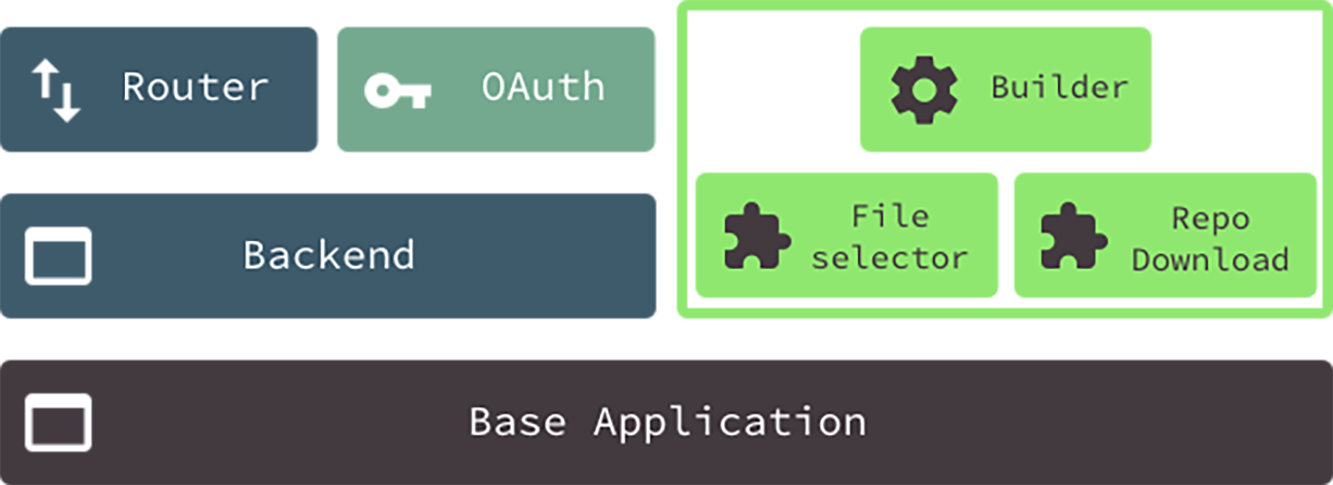
\includegraphics[width=0.9\textwidth]{application_structure.png}
    \caption{A graphic showing the base structure of the implemented application.\\ The \emph{base application} layer serves as foundation, containing necessary libraries for implementing the \emph{HTTP} specifications. The \emph{routing} and \emph{OAuth} layer are responsible for authenticated requests to the endpoints, while the \emph{builder package} is designed as a partly autonomous, loosely coupled rendering service.}
    \label{fig:application_structure}
\end{figure}
%

A basic approach of the project structure may be seen in fig. \ref{fig:application_structure}. Although this might look still very abstract, the core packages are already clearly visible, while neither the access to the GitHub API, nor the access to the MongoDB is yet visualized.

The graphic can be interpreted as follows:

\begin{itemize}
  \item \emph{Base Application} -- The base structure, consisting of a Node.js environment, together with necessary supporting packages, such as a MongoDB driver and a GitHub API implementation.
  \item \emph{Backend} -- The Express.js ecosystem, responsible for controlling the HTTP subset.
  \item \emph{Router} -- The Express.js router instance, providing all the necessary endpoints for accessing the application's functions.
  \item \emph{OAuth} -- The authentication framework, as theoretically explained on p. \pageref{sec:foundation-express-oauth}.
  \item \emph{Builder} -- The main build pipeline package consisting of many small plugins for asynchronous handling the process from parsing the configuration to actually building the website.
\end{itemize}

\subsection{Basic setup}
The base application layer is more or less a Node.js stack, covering necessary support features, like reading environment variables or creating various instances of needed modules for the main application flow. It also cares for connecting the service to a MongoDB database, as well as providing a connection framework to the GitHub API.

Furthermore, it holds different database models for user registration, OAuth tokens and build logs. These models are necessary for maintaining a consistent structure on the database collections, thus avoiding custom value checks after fetching entries. Using \emph{Mongoose}\footnote{\url{http://mongoosejs.com} -- Mongoose, ``elegant mongodb object modeling for node.js''}, additional features like manipulation functions and automatic population may be used without depending on other toolsets. One example would be the automatic hashing and comparison of passwords, which is enabled using \emph{pre} hooks on schemas at a certain event (e.g. ``save'')\footnote{\url{http://mongoosejs.com/docs/api.html\#schema_Schema-pre} -- ``Pre'' hook documentation for MongooseJS.}.

\subsubsection{Express.js}
On top of the base application layer, an Express.js setup works as a REST API service. It is configured as first instance in the application's main entry point and is bootstrapped right after the launch of the project. Extending the core module of Express is easy due to the built-in middleware pluggability. A middleware function may get added to the application by binding it to an instance of the app object using an \texttt{app.use()} call \cite{ExpressMiddleware}.

One of the additional middlewares used to extend the app instance is a logging mechanism called ``morgan''\footnote{\url{https://github.com/expressjs/morgan} -- Morgan repository on GitHub.}, which allows a fully customizeable output format for logging HTTP requests and the duration until a response was sent. Another important extension is ``method-override''\footnote{\url{https://github.com/expressjs/method-override} -- Method-override repository on GitHub.}. This module allows the consideration of a \emph{X-HTTP-Method-Override} field in the request header, sent by clients, which are not supporting request types like PUT or DELETE.

\subsubsection{Router}
The middleware concept is designed as a sequential flow of callback functions. Once a request is coming in, the instance is forwarding the data from middleware to middleware until either a response is returned and the middleware chain gets interrupted, or no additional function is left and the instance throws an error.

Thus, the routing mechanism is nothing more than a built-in middleware of Express. It allows for dividing incoming requests based on their URL structure and subsequently assigning them to their respective predefined tasks. These functions again may behave like middleware functions (e.g. for checking authorization, including abstracted functions, imposing pre-conditions, etc\ldots) and therefore expand the callback cycle by additional functionality \cite{ExpressRouter}.

\subsubsection{Authentication}
Several routes require authentication before being able to access, as a consequence, an automated mechanism handling all necessary steps for securely exchanging user details is inserted in front of the respective routes. Before doing so, the OAuth stack has been implemented -- the \emph{OAuth2orize} package provides an authorization server toolkit for setting up a service implementing the OAuth 2.0 protocol.

The skeleton coming with the package needs to be configured based on the current project's setup, then the instance exposes a middleware, which may be mounted in certain routes \cite{OAuth2orizeGitHub}. After this has happened, the use of the framework may divide the routing configuration into fully accessible routes on the one hand and routes with limited access on the other hand:

\lstinputlisting[caption={A basic router configuration showing the use of an authorization service as a middleware, thus dividing the routes into fully accessible ones (\emph{/all}) and ones with limited access (\emph{/limited} and \emph{/secret}).}, language=JavaScript, label={list:oauth-routes}]{chapters/05-implementation/_support/oauth.js}

From this point on, the client has to provide an access token in the \emph{Authorization} HTTP header using the ``Bearer'' authentication scheme for gaining access \cite[5]{RFC6750}. The service will deny further processing if either an inexisting or already expired access token was provided. In this case, the client has to exchange his/her correct client credentials for a new access token on the authorization endpoint prior accessing the desired endpoint again \cite[41]{hardt2012oauth}.


\subsection{Build pipeline}
After the HTTP- and authentication service was built as a user interaction possibility for the upcoming build pipeline realization, the full extent of the necessary API endpoints needed to be defined. Since the OAuth 2.0 framework was already implemented and the access to the GitHub API was prepared as includeable module, only the endpoints responsible for managing and triggering builds, needed to be reserved for the final build service development.

\subsubsection{API integration}

%% Graphic of the first draft of the API
\begin{figure} % h-ere, t-op, b-ottom, p-age
    \centering
    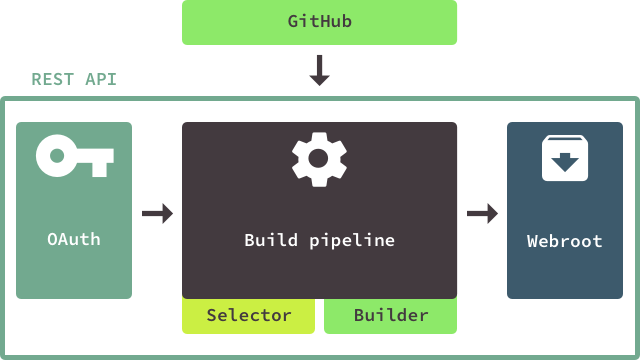
\includegraphics[width=0.9\textwidth]{buildpipeline-api.png}
    \caption{A graphic showing the first draft of the then proposed API cycle. At first the OAuth step should care for authentication, then the build pipeline should be initiated and orchestrate its services to interact with the GitHub API, select files to build and run the build task before saving a rendered version of the webroot, ready for deployment.}
    \label{fig:buildpipeline-api}
\end{figure}
%

From the first draft of an API cycle (as seen in fig. \ref{fig:buildpipeline-api}) to the final structure, a lot of details needed to be tidied up. This was mainly due to the complexity of the build pipeline itself, since one of the biggest challenges were to provide a real non-blocking event loop. By realizing such a non-blocking loop, the client receives an instant, intermediate response, instead of having to queue beforehand, and/or wait until the whole operation finishes. Furthermore, a recurring request for obtaining the build status was enabled using an own endpoint returning informations from the database entry.

The endpoints, which were implemented in favor of user projects, were the following:

\begin{itemize}
  \item \texttt{POST /api/project} -- Creates a project in the database, together with reference to its GitHub data.
  \item \texttt{POST /api/project/:owner/:repo/delete} -- Deletes all references to the project from the database.
  \item \texttt{POST /api/project/:owner/:repo/build} -- Trigger a new build cycle. Returns the reference to the database entry of its build log.
  \item \texttt{GET /api/project/:owner/:repo/status} -- Get the status of the latest build (pending, failed, success).
  \item \texttt{GET /api/project/:owner/:repo/download} -- Download the latest successful build as tar.gz-archive. (e.g. for automated deployments)
\end{itemize}

\section{Engine}
\label{sec:engine}

The build pipeline engine basically wraps a common interface around the static site generator. Together with already mentioned supporting modules, it forms a nearly standalone ecosystem within a service, which happens to expose a REST API.

Other than pure HTTP services, the build engine not only has to cope with database queries -- its main purpose is to handle file input/output management based on various configurations, ideally asynchronous and possibily even in parallel. Especially the latter may cause trouble at some point, because of JavaScript's single threaded model. Though Node.js may handle asynchronous operations well, it requires its event loop to continue running, when non-blocking operations (like input/output) are executed concurrently. This differs heavily from other programming languages, which are likely to create additional threads for such kind of tasks \cite{NodejsBlockingNonblocking}.

\subsection{Asynchronous work}
Possibly one of the most important requirements of the project is to work with asynchronous calls, as well as processing them as performant as possible. As already explained, the API depends on a significant variety of tasks for fetching data to create an instance of the build pipeline according to a certain configuration.

Most of them are realized using the JavaScript Promise API, where on the one hand subsequently nesting callback functions are avoided and on the other hand, various \emph{then}-functions are not only getting chained to each other (``Promise chain''), but also returning a Promise themself \cite{MDNPromise}. This allows to keep an asynchronous flow in the same block -- some operations even allow handling more than one asynchronous function concurrently within a Promise construct.

As a result, all API calls to GitHub are realized using Promises -- as a matter of fact, the contained \emph{then}-functions are acting as necessary backbone, as the returned data often needs to be altered or even merged with the response of a second, concurrent request. One example would be the comparison of the existing file tree versus the affected files by the commit range.

\subsection{Child processes}
For keeping the API responsive to requests while a build process is running, it makes sense to decouple the heavy rendering task into an own process (``Child process''). The child process will balance the work load, so that the rendering will happen in its own V8-process on an additional processor core \cite[335]{cantelon2017node}, only able to communicate to the host process via emitting events on its built-in communication channel \cite{NodejsChildProcesses}. The host process will reside in its initial thread and only receive a message, if the child process emits one or exited -- therefore enough information will be distributed to keep the project's status in the database up to date.

There is a critical thing to consider though; since every child process gets equipped with an own memory and V8 instance, constantly allocating resources by spawning a large amount processes may lead to unexpected server crashes \cite{NodejsChildProcesses}. Virtual private servers (\emph{VPS}) with a significant amount of RAM, as well as up to 20 processor cores and more will handle such heavy tasks of course better than local machines with often less than 4 cores, but also have to be managed well in terms of resource usage. Every child process is likely to occupy a minimum of 10 megabytes of RAM by default -- though this amount surely increases. The final extent is based on the task it has to handle \cite{RobinsonNodeCluster}.

\subsection{Storage}
Because of the fact, that the project requires different stages of every repository to be stored for making use of caching, a significant amount of data has to be stored for quick access. To not loose track on the constantly growing extent, it possibly would be best to export them to long-lasting storage services like Amazon S3 buckets\footnote{\url{https://aws.amazon.com/de/s3/} -- Amazon's S3 cloud storage service.} -- however, due to the many locally hosted services (first and foremost the REST API), the decision was made in favor of also storing repository data locally in the mean time during development.

The first kind of data to outsource would surely be the rendered archive, containing the webroot. As this needs to be accessed at all time, a downtime is simply not acceptable and a constant uptime cannot be guaranteed on a service like this, unless it is also run on multiple failsafe instances around the globe.

\subsection{Realization}
After the necessary technologies for providing a non-blocking event flow were defined, the build pipeline module set could be brought in shape. Together with the wrapping REST API and the predefined endpoints (see ch. \ref{sec:structure-buildpipeline} on p. \pageref{sec:structure-buildpipeline}f), the main entry point should be able to carry the heavy load of instantiating the static site generator, as well as fetching data from GitHub. Furthermore, it should act as control interface for managing the internal communication between Metalsmith and the API.

%% Graphic of the finished workflow of the build pipeline
\begin{figure} % h-ere, t-op, b-ottom, p-age
    \centering
    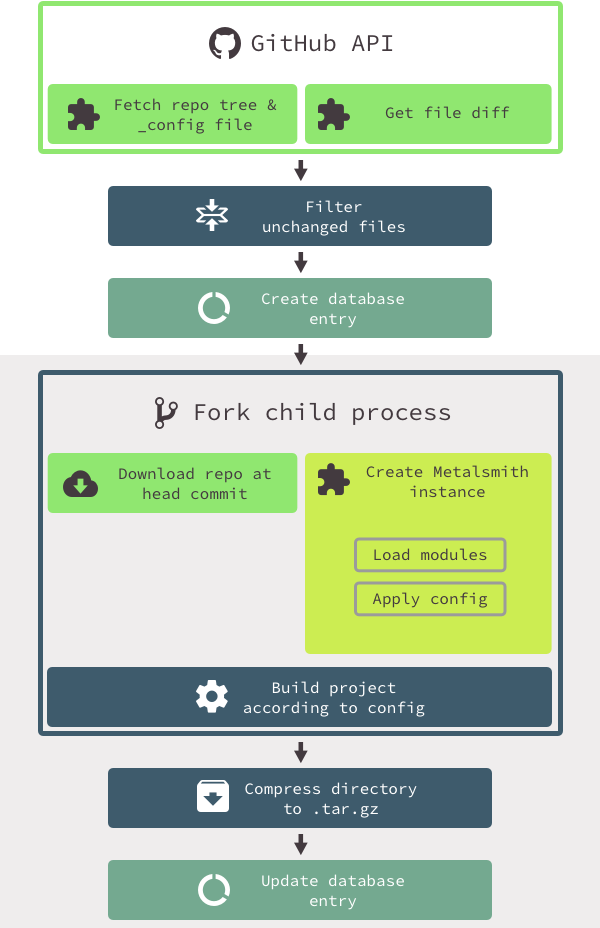
\includegraphics[width=0.75\textwidth]{application_flow.png}
    \caption{A graphic showing the main application flow of the build pipeline from top to bottom. At first, the \emph{repo tree} and \emph{file diff} are fetched from the GitHub API in parallel. After file filtering and creating a database entry, a child process is forked, which cares for executing the heavy tasks for building. After a successful build, the resulting files are compressed into a \emph{tar.gz} archive, then the database entry is updated accordingly. Afterwards, the child process is terminating gracefully.}
    \label{fig:application-flow}
\end{figure}
%

As seen in fig. \ref{fig:application-flow}, much of the build pipeline's workflow actually happens without the user knowing about (grayish area). Basically the only thing happening before sending an HTTP response, is the parsing of the configuration file, as well as filtering files, affected by the commit range. If both succeeds, the database entry is created and the user may then query the API for getting to know the current status, while the main task possibly is still running in a forked child process. So, the REST API stays responsive the whole time during build, without causing any lack of performance.

\subsubsection{Forking a child process}
According to the Node.js documentation, the \texttt{child\_process.fork()}-function is used specifically to spawn new Node.js processes. This means, that every child process creation happens without breaking the event loop of the parent process \cite{NodejsChildProcesses}. Therefore this step is crucial before invoking any heavy task, which may result in blocking the API's responsiveness to handle additional HTTP requests.

Since the sub process is completely decoupled from the main task, it likely will not share the same current working directory as its parent process. Whenever that happens, a \emph{cwd} option may be set in the configuration object upon fork \cite{NodejsChildProcesses}. The Metalsmith instance requires this feature, as every repository it will be working on is nested in a certain sub folder in the project's file tree. Most of the Metalsmith plugins are designed to only work in the actual CWD, unlike its API initially proposed (see line 5 in Listing \ref{list:metalsmith} on p. \pageref{list:metalsmith}) \cite{MetalsmithRepository}.

What happens in the child task although is the following; the respective repository archive is being fetched from the GitHub API -- this happens in parallel to setting up the build pipeline:

\begin{enumerate}
  \item Creating a Metalsmith instance by setting the global API options according to the global configuration object, provided by the parent process.
  \item Filter required Metalsmith module names from the configuration object
  \item Sequentially invoke the modules to the Metalsmith instance
  \begin{enumerate}
    \item Check if the current module is already available in the main project's node modules folder,
    \item append it by default,
    \item or catch any error by appending the module name into an array of yet missing node modules.
    \item \texttt{npm install} the missing modules and repeat.
  \end{enumerate}
  \item Return the completed Metalsmith instance to the child process.
\end{enumerate}

All that is still missing, is waiting until both tasks (archive fetching, build pipeline setup) have succeeded, before the \texttt{build()}-function is ready to be triggered and the rendering process will be initiated. No matter if it fails or succeeds, the parent process receives a message containing necessary build information in any case.

\subsubsection{Finishing the task}

